Agents need to agree on multiple decisions, and therefore leader has to be elected among the agents. Leader will be responsible of generating and announcing the map, and up streaming data about the swarm to other services(backend). Main algorithm behind leader election is presented on the figure \ref{fig:election_logic}. 

\begin{figure}[H]
    \centering
    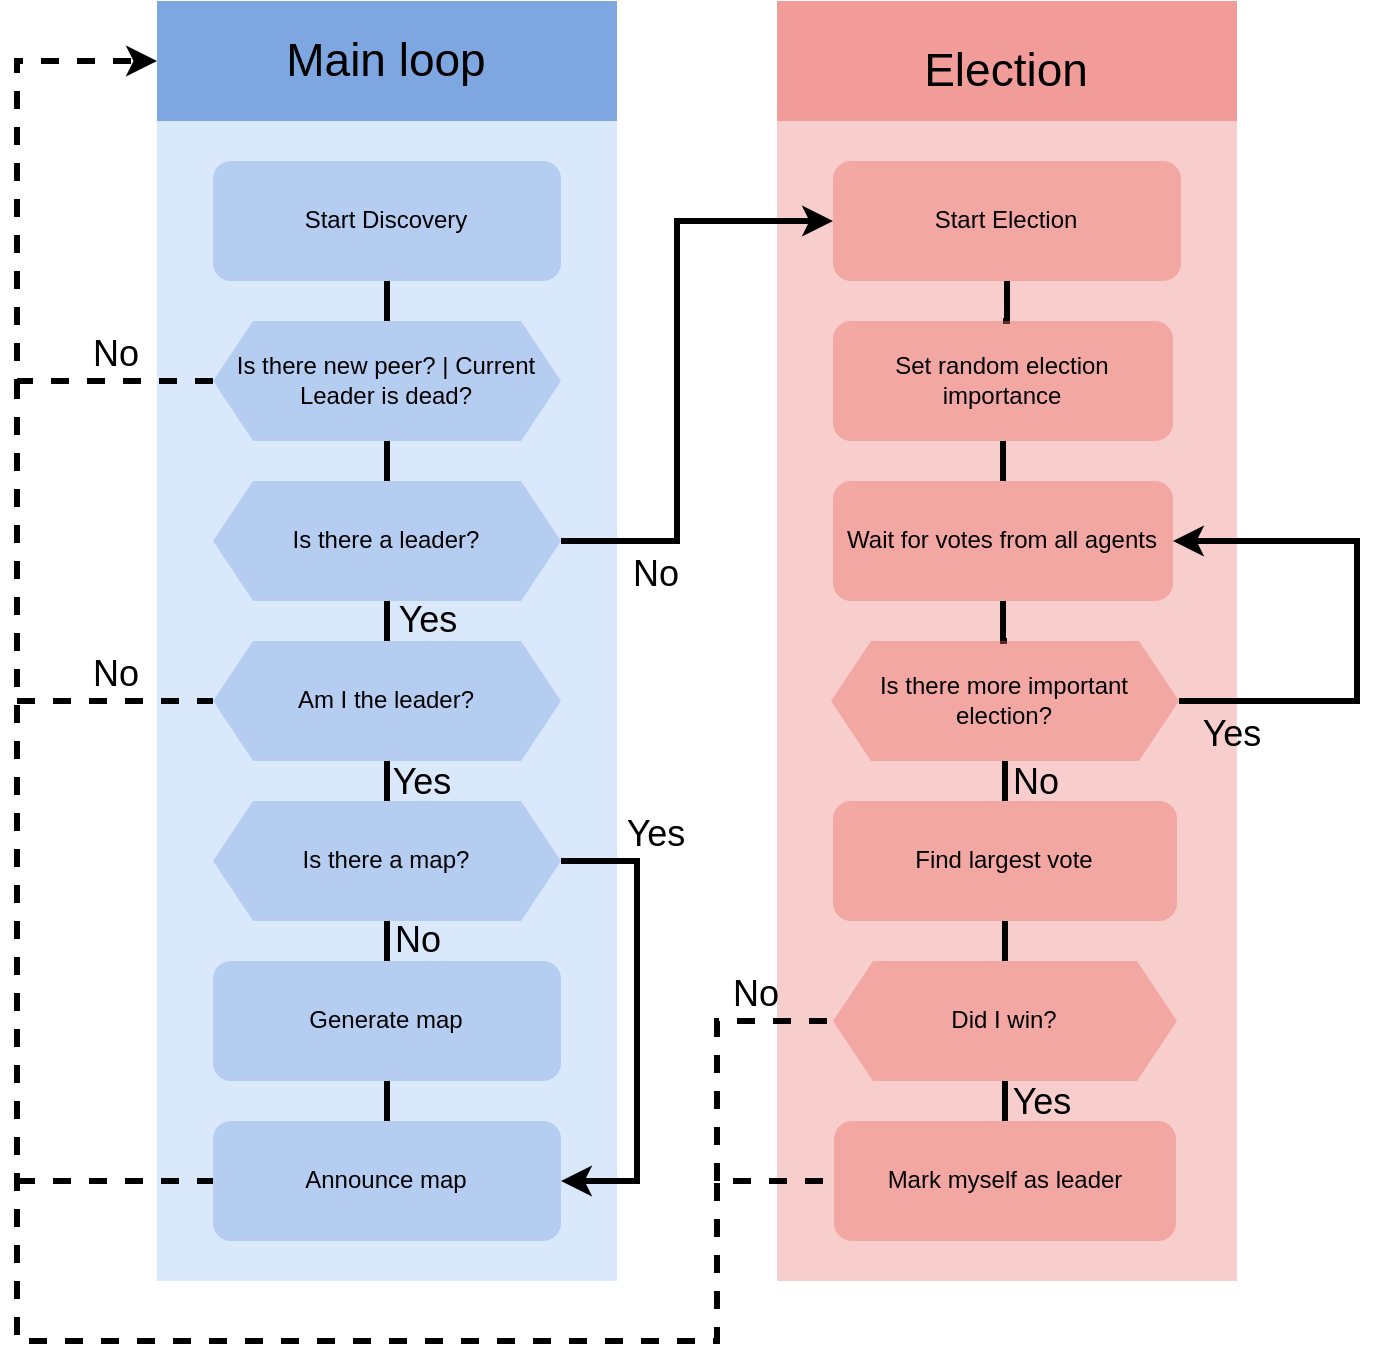
\includegraphics[width=0.8\textwidth]{pictures/election_logic.png}
    \caption{ Election logic}
    \label{fig:election_logic}
\end{figure}

Election will be triggered when new peer will be discovered or current leader is dead(not able to reach). Additional requirement is that there is no living leader already elected. After those checks are triggered, agent will send a message to other to start election, with random number signalizing importance of the election. Multiple elections can be started at the same time by multiple agents.

After starting an election, agent will be waiting to receive votes from all other agents, unless it will receive message about more important(higher number) election started. Once all the votes(randomly generated) are received agent with highest vote wins the election and will announce itself a leader, and other agents will accept it as a leader. To avoid the collision of both votes and  election importance number, those has to be set to large number.